\documentclass{article}
\usepackage[backend=biber]{biblatex}
\usepackage[german]{babel}
\usepackage{graphicx}
\usepackage{enumitem}
\graphicspath{ {./img/} }

\setlength{\parindent}{0pt}

\bibliography{ByzantinischeFehler}

\title{Byzantinische Fehler}
\author{Matthias Reumann}
\date{\today}

\begin{document}

\maketitle

\newpage

\tableofcontents

\newpage

\iffalse
\section{Byzantinische Fehler}

\subsection{Definition}

Byzantinische Fehler treten in verteilten Systemen auf, 
wenn fehlerhafte Nachrichten von einem Knoten versendet werden, 
die von der Struktur und vom Inhalt nicht von fehlerfreien
unterscheidet werden können. \cite{esraberlin} 

\medskip 

Den Namen hat diese Fehlerklasse im Jahr 1982 von Lamport et. al. im 
Papier \textit{The Byzantine Generals Problem} erhalten.\cite{generals}
In diesem werden Byzantinische Fehler durch das abstrakte Beispiel 
der Byzantinischen Generäle beschrieben, dass im Abschnitt \ref{sec:generals} genauer erläutert wird.

\subsection{Problem}

Man stelle sich $n$ unabhängige Sensoren eines Notbremsassistenten vor, die miteinander kommunzieren.
Dabei werden nur Nachrichten \textit{STOP} oder \textit{OK} gesendet. Sobald einer der Sensoren, 
einen Wert misst, der unter eine Schranke $s$ fällt, teilt er dies den anderen $n-1$ Sensoren mit.

\medskip 

Hierbei ist die Aufgabe der Sensoren, eine gemeinsame Entscheidung zu fällen, ob gebremst werden soll. 
Oftmals wird dafür die absolute Mehrheit der Nachrichten verwendet. Diese Vorgehensweise funktioniert 
solange, bis ein Sensor fehlerhafte Informationen übermittelt, da keiner Sensoren die Fähigkeit besitzt die 
erhaltenen Informationen auf ihre Richtigkeit zu prüfen. Das könnte zu einer Fehlentscheidung führen 
und in Beispielen, wie dem Notbremsassistenten, fatale Folgen haben. 

\medskip 

Ein Beispiel eines solchen Byzantinischen Fehlers kann in Abbildung \ref{fig:example} gesehen werden. 

\begin{figure}[h]
    \centering
    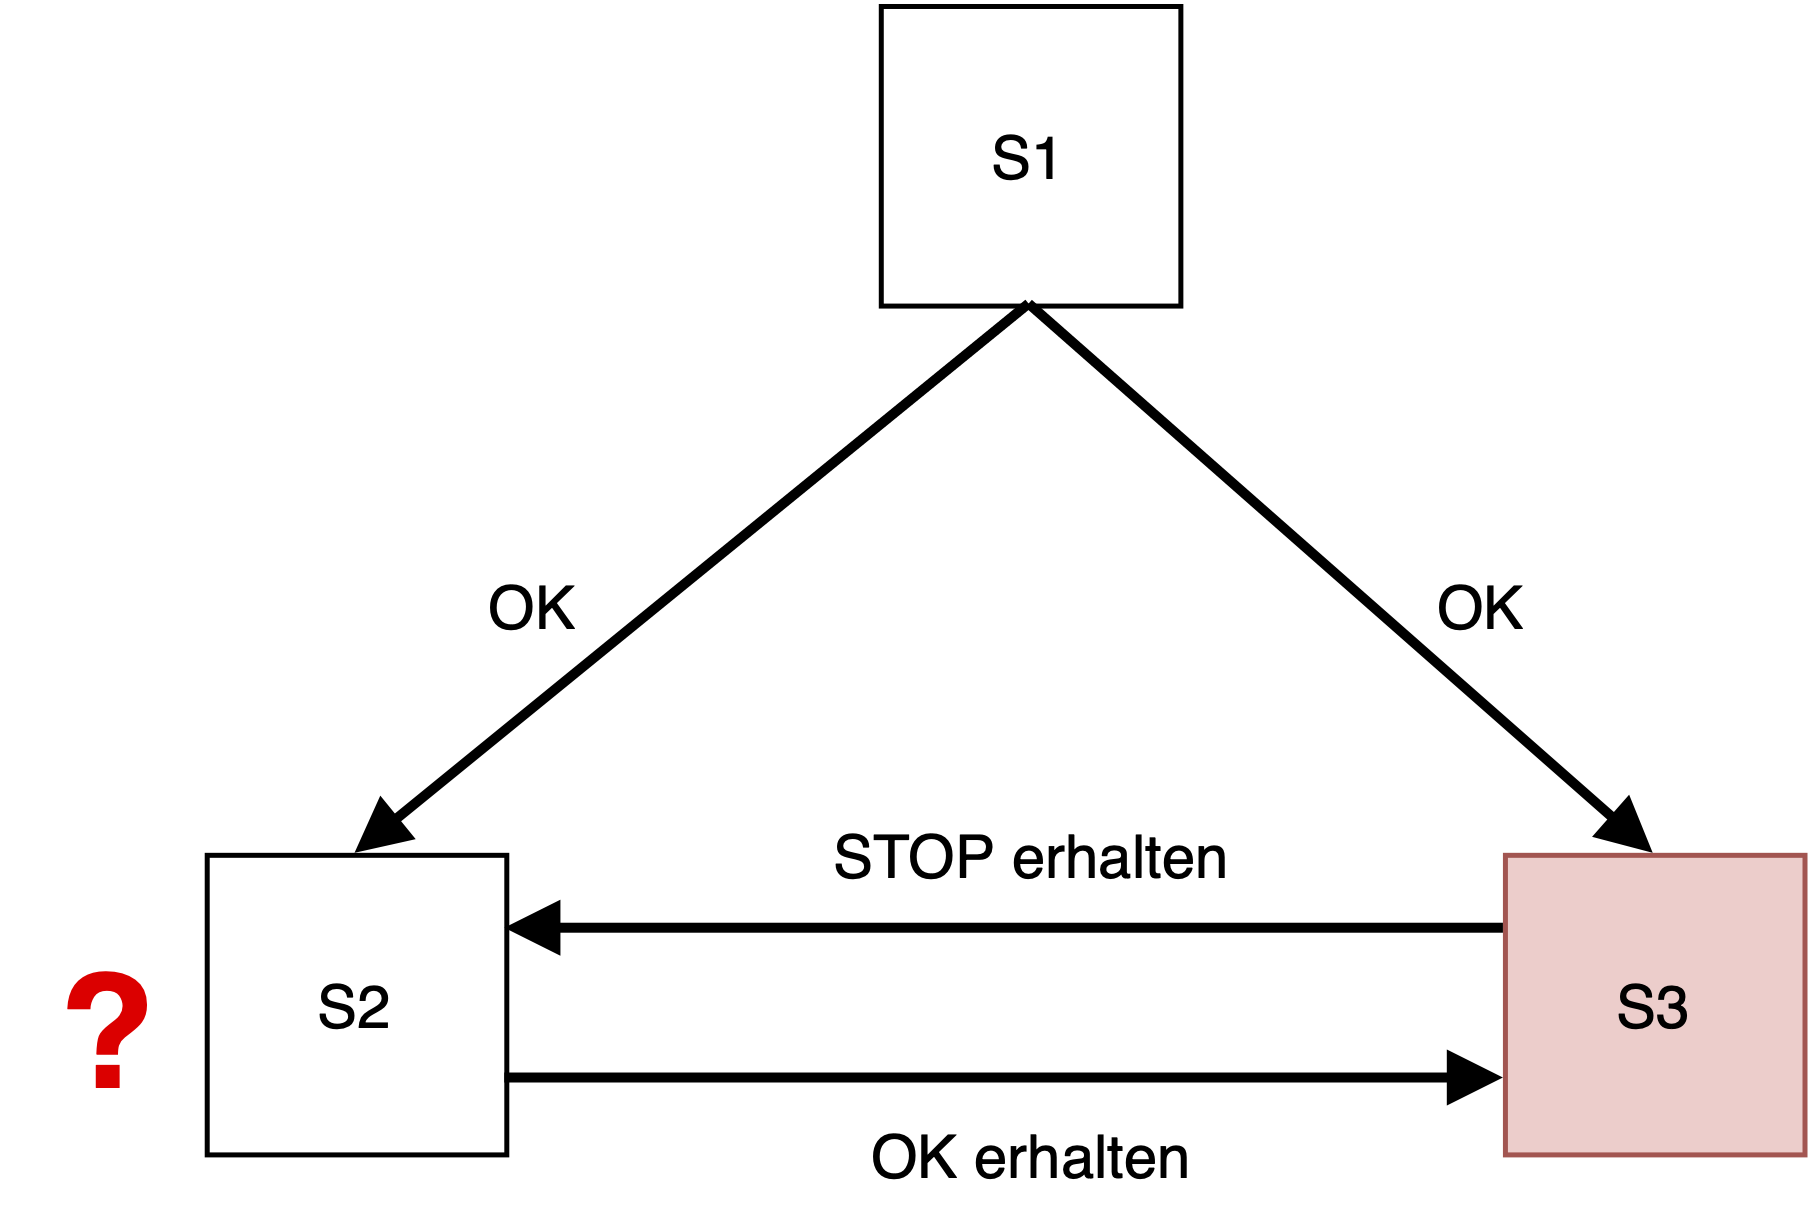
\includegraphics[width=0.7\textwidth]{byz-sensor-example.png}
    \caption{Sensornetzwerk mit fehlerhaftem Sensor 3. Für Sensor 2 ist es nicht möglich eine eindeutige Entscheidung zu treffen.}
    \label{fig:example}
\end{figure}

\medskip 

\fi

\section{Problem der byzantinischen Generäle}
\label{sec:generals}

Mehrere Truppen mit jeweils einem General umzingeln eine feindliche Stadt und 
kommunizieren direkt über Boten miteinander. 
Jeder der Generäle beobachtet den Feind und schlussendlich müssen die Generäle 
eine gemeinsame Entscheidung treffen. Jedoch kann es unter den Generälen Verräter geben,
deren Ziel es ist eine gemeinsame Entscheidung der loyalen Generäle zu unterbinden. 

\medskip 

Die Generäle müssen einen Algorithmus finden der garantiert, dass

\begin{enumerate}[label=(\alph*)]
\item Alle loyalen Generäle die gleiche Entscheidung treffen 
\item Eine geringe Anzahl an Verrätern die loyalen Generäle nicht zu einer Fehlentscheidung führt
\end{enumerate}

Eine Entscheidung unter den Generälen wird gefällt 
indem jeder General den Feind beobachtet und seine
Informationen an die anderen Generäle weitergibt. \textit{v(i)} ist die 
Nachricht gesendet vom $i$.ten General. Jeder General erhält die Nachrichten 
\textit{v(1)} bis \textit{v(n)}, wobei $n$ die Anzahl der Generäle darstellt. 
Die finale Entscheidung wird durch die absolute Mehrheit der Werte dieser Nachrichten
bestimmt. Allerdings könnte es sein, dass loyale Generäle unterschiedliche \textit{v(i)}
erhalten, da ein Verräter unterschiedliche Werte zu unterschiedlichen Generälen sendet, 
was widerum Punkt A widerspricht. 

Deshalb müssen sogennante \textit{interactive consistency}-Bedingungen gelten.
Ein führender General, auch "Commander" gennant, sendet einen Befehl an seine $n - 1$ Leutnant 
Generäle so, dass:

\smallskip 

\begin{tabular}{l l}
IC1 & Alle loyalen Leutants den gleichen Befehl ausführen \\
IC2 & Wenn der Commander loyal ist, dann befolgt jeder loyale Leutnant seinen Befehl
\end{tabular}

\iffalse

\medskip 

Dabei kann durch Widerspruch bewiesen werden, dass die Anzahl der Generäle $n$ größer als $3m + 1$ sein muss, wobei $m$ die Anzahl der 
Verräter ist.

\begin{figure}[h]
    \centering
    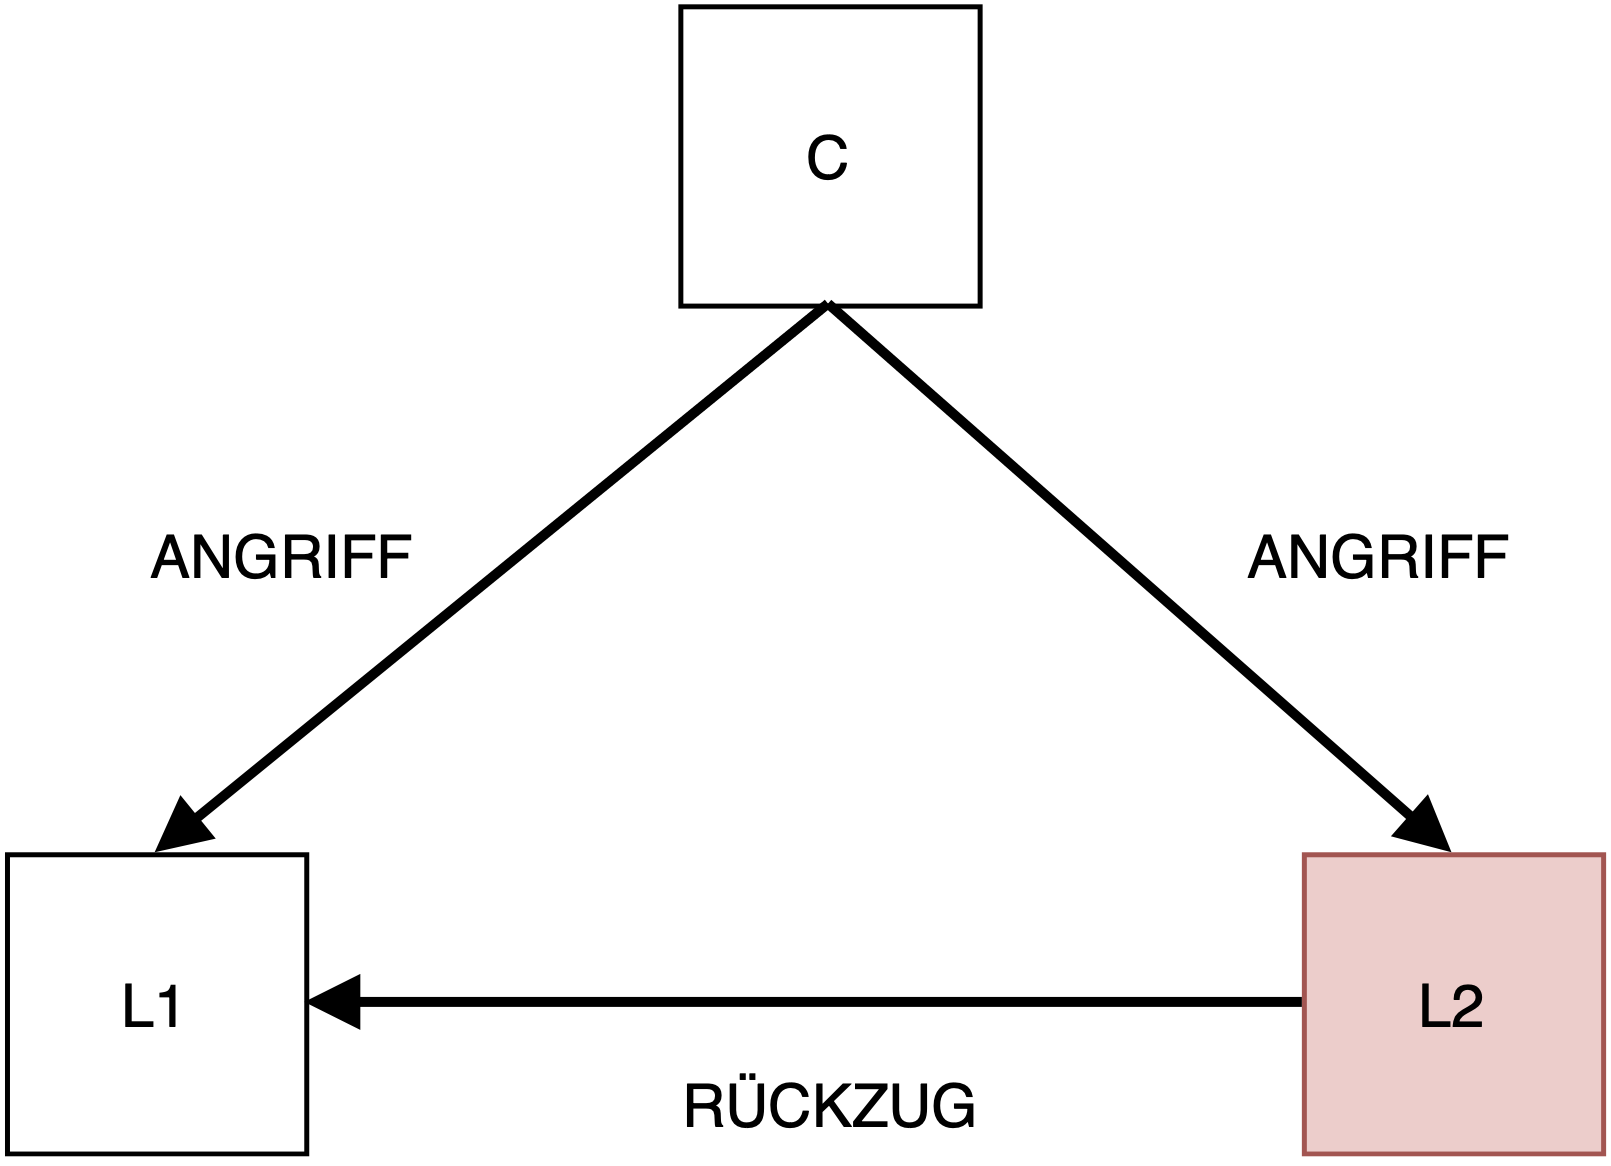
\includegraphics[width=0.45\textwidth]{general1.png}
    \hfill
    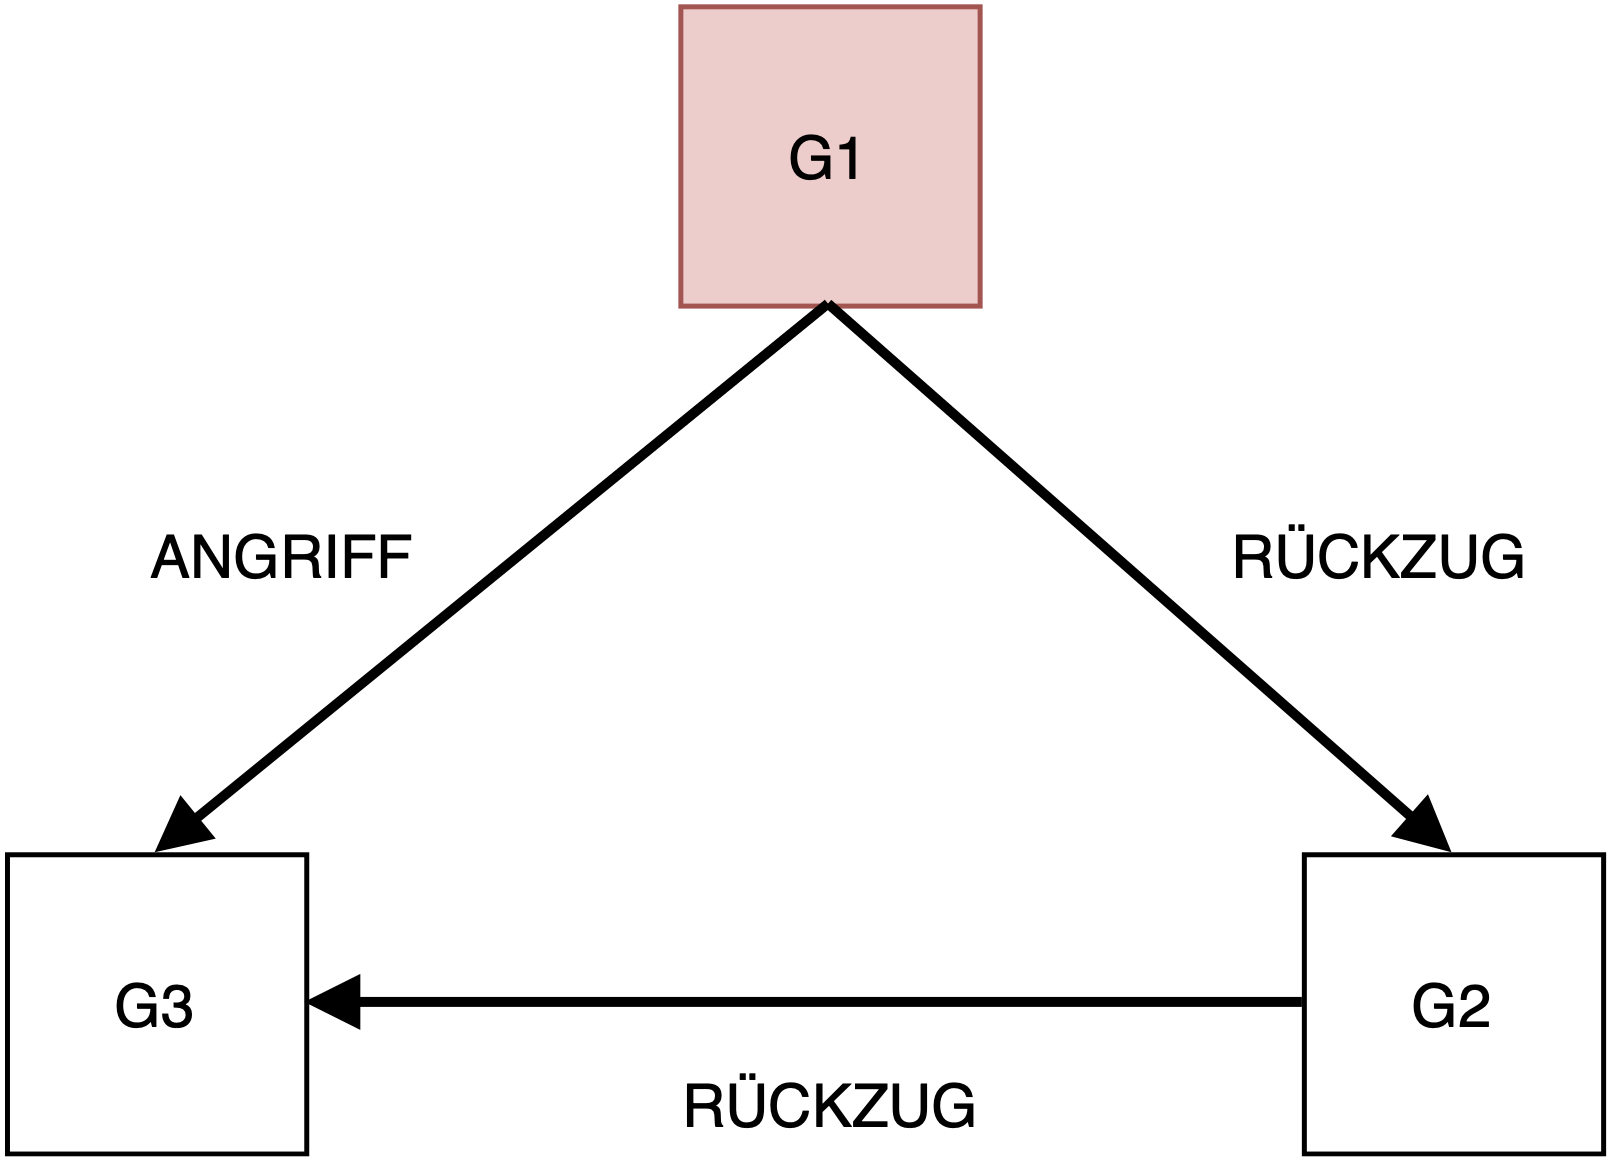
\includegraphics[width=0.45\textwidth]{general2.png}
    \caption{Zeigt, dass es nicht möglich ist eine Lösung zu finden, wenn ein Drittel der Generäle, Verräter sind. 
            Der Verräter ist in beiden Abbildungen rot markiert.}
    \label{fig:generals}
\end{figure}

\medskip 

General G1 stellt in den beiden Beispielen den Commander dar, der Befehle an seine Leutants G2 und G3 schickt. 
In beiden Fällen möchte G3 erfahren, welche Nachricht G2 von G1 erhalten hat. Hierbei spielt es keine Rolle ob G1 oder G2 
der Verräter ist, denn in beiden Fällen kann G3 keine eindeutige Entscheidung treffen.  

\subsection{Lösung}

\subsection{Kritik}

Der OM-Algorithmus ist sehr aufwendig. Er ist praktisch nicht für große $n$ und $m$ einsetzbar.  

\subsection{Beispiel}

\newpage 

\printbibliography

\fi


\end{document}